%--------------------------------------------------------------------%
%
% Title         : Postgraduate Thesis LaTex template
% Author        : Ravi Vendra Rishika <ravi.vendra.rishika@gmail.com>
%
% Page          : Main TeX
%
% It is developed especially for postgraduate students of :
%   Department of Informatics
%   Faculty of Intelligent Electrical and Informatics Technology
%   Sepuluh Nopember Institute of Technology (ITS)
%   Surabaya, Indonesia.
%
% This LaTex template is intended to make students easier
% to write master's degree thesis in LaTex using specific
% Department of Informatics of ITS' format.
%
%--------------------------------------------------------------------%

\documentclass[11pt, a4paper, onecolumn, twoside, final, indonesian]{book}

%--------------------------------------------------------------------%
%
% Title         : Postgraduate Thesis LaTex template
% Author        : Ravi Vendra Rishika <ravi.vendra.rishika@gmail.com>
%
% Page          : Preambule (Import Library)
%
% It is developed especially for postgraduate students of :
%   Department of Informatics
%   Faculty of Intelligent Electrical and Informatics Technology
%   Sepuluh Nopember Institute of Technology (ITS)
%   Surabaya, Indonesia.
%
% This LaTex template is intended to make students easier
% to write master's degree thesis in LaTex using specific
% Department of Informatics of ITS' format.
%
%--------------------------------------------------------------------%

\special{papersize=210mm,297mm}

% Setting margin
% \usepackage[top=3cm,bottom=2.5cm,left=3cm,right=2.5cm]{geometry}
\usepackage[top=3.5cm,bottom=3cm,inner=4cm,outer=3cm]{geometry}

\usepackage{mathptmx}

% Judul bahasa Indonesia
\usepackage[indonesian]{babel}

%Includes "References" in the table of contents
\usepackage[nottoc]{tocbibind}

\usepackage[utf8]{inputenc}
\usepackage{graphicx, titling, blindtext, sectsty, chngcntr}
\usepackage{etoolbox, titlesec, parskip, watermark, eso-pic}
\usepackage[hidelinks]{hyperref}
\usepackage[pages=some]{background}
\usepackage{setspace}
\usepackage{xcolor, ragged2e}

\usepackage{amsmath, csquotes}

% Format citation
% \usepackage[style=authoryear-ibid,backend=biber]{biblatex}
% \usepackage[backend=biber,style=numeric]{biblatex}
% \usepackage[backend=bibtex,citestyle=authoryear]{biblatex}
\usepackage{natbib}

% \usepackage[T1]{fontenc}
% \usepackage{tgbonum}

\renewcommand{\baselinestretch}{1.5}

\chapterfont{\centering \Large}
\titleformat{\chapter}[display]
  {\Large\centering\bfseries}
  {\chaptertitlename\ \thechapter}{0pt}
    {\Large\bfseries\uppercase}

\setcounter{secnumdepth}{3}

\makeatletter

\makeatother

\counterwithin{figure}{section}
\counterwithin{table}{section}


\makeatletter

\makeatother

% \SetWatermarkLightness{0.9}
% \SetWatermarkText{\includegraphics[angle=-45]{src/resources/its-thesis-cover.png}

% \newcommand\BackgroundPic{
%     \put(0,0){
%         \parbox[b][\paperheight]{\paperwidth}{
%             \vfill
            
%             \centering
%             \includegraphics[width=\paperwidth,height=\paperheight,keepaspectratio]{src/resources/its-thesis-cover.png}
            
%             \vfill
%         }
%     }
% }

% IEEE Bibliography Style
% \bibliographystyle{abbrvnat}

% Harvard Bibliography Style
\bibliographystyle{agsm}

\setcitestyle{authoryear, open={(},close={)}}

\backgroundsetup{
    scale=1,
    color=black,
    opacity=1.0,
    angle=0,
    contents={%
        
\includegraphics[width=\paperwidth,height=\paperheight]{src/resources/its-thesis-cover-without-logo.png}
    }%
}

\begin{document}

    % \AddToShipoutPicture*{\BackgroundPic}
    \BgThispage
    
    % New variables defined here
    \newcommand\titleID{TESIS MAHASISWA DEPARTEMEN TEKNIK INFORMATIKA INSTITUT TEKNOLOGI SEPULUH NOPEMBER (DALAM BAHASA INDONESIA)}
    \newcommand\titleEN{POSTGRADUATE STUDENT THESIS OF INFORMATICS DEPARTMENT OF SEPULUH NOPEMBER INSTITUTE OF TECHNOLOGY (IN ENGLISH)}

    \newcommand\authorName{Nama Mahasiswa}
    \newcommand\authorNRP{60xxxxxxxx}
    
    \newcommand\firstSupervisorName{Dosen Pembimbing ke-1 (Lengkap)}
    \newcommand\firstSupervisorNameShort{Dosen Pembimbing ke-1 (Singkat)}
    \newcommand\firstSupervisorNIP{20xxxxxxxx}
    \newcommand\firstSupervisor{
        \firstSupervisorName \\
        NIP \> : \firstSupervisorNIP
    }
    
    \newcommand\secondSupervisorName{Dosen Pembimbing ke-2 (Lengkap)}
    \newcommand\secondSupervisorNameShort{Dosen Pembimbing ke-2 (Singkat)}
    \newcommand\secondSupervisorNIP{20xxxxxxxx}
    \newcommand\secondSupervisor{
        \secondSupervisorName \\
        NIP \> : \secondSupervisorNIP
    }
    
    \newcommand\firstExaminerName{Dosen Penguji ke-1 (Lengkap)}
    \newcommand\firstExaminerNameShort{Dosen Penguji ke-1 (Singkat)}
    \newcommand\firstExaminerNIP{20xxxxxxxx}
    \newcommand\firstExaminer{
        \firstExaminerName \\
        NIP \> : \firstExaminerNIP
    }
    
    \newcommand\secondExaminerName{Dosen Penguji ke-2 (Lengkap)}
    \newcommand\secondExaminerNameShort{Dosen Penguji ke-2 (Singkat)}
    \newcommand\secondExaminerNIP{20xxxxxxxx}
    \newcommand\secondExaminer{
        \secondExaminerName \\
        NIP \> : \secondExaminerNIP
    }
    
    \newcommand\thirdExaminerName{Dosen Penguji ke-3 (Lengkap)}
    \newcommand\thirdExaminerNameShort{Dosen Penguji ke-3 (Singkat)}
    \newcommand\thirdExaminerNIP{20xxxxxxxx}
    \newcommand\thirdExaminer{
        \thirdExaminerName \\
        NIP \> : \thirdExaminerNIP
    }

    \newcommand\finalExamDay{-}
    \newcommand\finalExamDate{-}
    \newcommand\finalExamPlace{Online}
    
    \newcommand\postgraduateProgram{Program Magister}
    \newcommand\postgraduateCourseClass{Komputasi Berbasis Jaringan}
    \newcommand\postgraduateDepartment{Departemen Teknik Informatika}
    \newcommand\postgraduateFaculty{Fakultas Teknologi Elektro dan Informatika Cerdas}
    \newcommand\postgraduateUniversity{Institut Teknologi Sepuluh Nopember}
    \newcommand\postgraduateCity{Surabaya}
    \newcommand\postgraduateYear{\the\year{}}
    
    % Custom variable

    %Basic configuration
    \author{
        \authorName \\
        NRP \> : \authorNRP
    }
    \date{}
    \title{
        \titleID
    }

    \pagenumbering{roman}
    \setcounter{page}{1}

    %--------------------------------------------------------------------%
%
% Title         : Postgraduate Thesis LaTex template
% Author        : Ravi Vendra Rishika <ravi.vendra.rishika@gmail.com>
%
% Page          : Cover
%
% It is developed especially for postgraduate students of :
%   Department of Informatics
%   Faculty of Intelligent Electrical and Informatics Technology
%   Sepuluh Nopember Institute of Technology (ITS)
%   Surabaya, Indonesia.
%
% This LaTex template is intended to make students easier
% to write master's degree thesis in LaTex using specific
% Department of Informatics of ITS' format.
%
%--------------------------------------------------------------------%

\clearpage

\newgeometry{top=1.5cm,bottom=3cm,right=3cm,left=3cm}

\pagestyle{empty}

\begin{flushleft}
    \color{white}
    
    \begin{figure}[h]
        % \centering
        
\includegraphics[width=3.5cm, height=3.5cm]{src/resources/its-logo.png}
    \end{figure}
    
    \vspace{4.5cm}
    
    {\fontfamily{lmss}\selectfont \Large \bfseries \MakeUppercase
        PROPOSAL TESIS
    }
    
    \vspace{25pt}
   	
    {\fontfamily{lmss}\selectfont \LARGE \bfseries \MakeUppercase
        \thetitle
    }
  	
  	\vspace{25pt}

    \begin{singlespace}
   	    {\fontfamily{lmss}\selectfont \Large \bfseries
   	        \theauthor
        }
    \end{singlespace}
    
    \vspace{25pt}

    \begin{singlespace}
   	    {\fontfamily{lmss}\selectfont
            \large \bfseries Dosen Pembimbing :

            \begin{enumerate}
                \item \firstSupervisor
                \item \secondSupervisor
            \end{enumerate}
        }
    \end{singlespace}
    
    \vspace{25pt}

    \begin{singlespace}
   	    {\fontfamily{lmss}\selectfont
            \large \bfseries \MakeUppercase {
            	\postgraduateProgram \\
                Rumpun Mata Kuliah \postgraduateCourseClass \\
                \postgraduateDepartment \\
                \postgraduateFaculty \\
                \postgraduateUniversity \\
                \postgraduateCity \\
                \postgraduateYear
            }
        }
    \end{singlespace}

\end{flushleft}

\restoregeometry

\clearpage


    \pagestyle{plain}
    
    %--------------------------------------------------------------------%
%
% Title         : Postgraduate Thesis LaTex template
% Author        : Ravi Vendra Rishika <ravi.vendra.rishika@gmail.com>
%
% Page          : Blank Page (intended first for empty Even page)
%
% It is developed especially for postgraduate students of :
%   Department of Informatics
%   Faculty of Intelligent Electrical and Informatics Technology
%   Sepuluh Nopember Institute of Technology (ITS)
%   Surabaya, Indonesia.
%
% This LaTex template is intended to make students easier
% to write master's degree thesis in LaTex using specific
% Department of Informatics of ITS' format.
%
%--------------------------------------------------------------------%

\clearpage

\begin{center}
    \smallskip

    \normalsize \normalfont
    
    \topskip 0pt
    
    \vspace*{\fill}
    \textit{Halaman ini sengaja dikosongkan.}
    \vspace*{\fill}
\end{center}

\clearpage

    
    %--------------------------------------------------------------------%
%
% Title         : Postgraduate Thesis LaTex template
% Author        : Ravi Vendra Rishika <ravi.vendra.rishika@gmail.com>
%
% Page          : Approval
%
% It is developed especially for postgraduate students of :
%   Department of Informatics
%   Faculty of Intelligent Electrical and Informatics Technology
%   Sepuluh Nopember Institute of Technology (ITS)
%   Surabaya, Indonesia.
%
% This LaTex template is intended to make students easier
% to write master's degree thesis in LaTex using specific
% Department of Informatics of ITS' format.
%
%--------------------------------------------------------------------%

\clearpage

\addcontentsline{toc}{chapter}{Lembar Pengesahan}

\newgeometry{top=3.5cm,bottom=3cm,inner=3.5cm,outer=3.75cm}

\begin{center}
    \smallskip

    \Large \MakeUppercase{
        \textbf{Lembar Pengesahan \\
        Proposal Tesis}
    }

    \vspace{15pt}

    \large

    \begin{flushleft}
        \setlength{\tabcolsep}{12pt}
        \begin{tabular}{p{0.15\linewidth} p{0.85\linewidth}}
            Judul       & : \thetitle \\
            Mahasiswa   & : \authorName \\
            NRP         & : \authorNRP
        \end{tabular}
    \end{flushleft}
    
    \vspace{25pt}

    \large Telah diseminarkan pada :
    
    \begin{flushleft}
        \setlength{\tabcolsep}{12pt}
        \begin{tabular}{p{0.15\linewidth} p{0.85\linewidth}}
            Hari        & : \finalExamDay \\
            Tanggal     & : \finalExamDate \\
            Tempat      & : \finalExamPlace
        \end{tabular}
    \end{flushleft}
    
    \vspace{25pt}
    
    \large Mengetahui / Menyetujui
    
    \begin{flushleft}
        \setlength{\tabcolsep}{12pt}
        \begin{tabular}{p{0.45\linewidth} p{0.55\linewidth}}
            \textbf{Dosen Penguji :} & \textbf{Dosen Pembimbing :} \\
            1. & 1. \\
            & \\
            \firstExaminerNameShort & \firstSupervisorNameShort \\
            NIP \> : \firstExaminerNIP & NIP \> : \firstSupervisorNIP \\
            2. & 2. \\
            & \\
            \secondExaminerNameShort & \secondSupervisorNameShort \\
            NIP \> : \secondExaminerNIP & NIP \> : \secondSupervisorNIP \\
            3. & \\
            & \\
            \thirdExaminerNameShort & \\
            NIP \> : \thirdExaminerNIP & \\
        \end{tabular}
    \end{flushleft}
\end{center}

\restoregeometry

\clearpage

    %--------------------------------------------------------------------%
%
% Title         : Postgraduate Thesis LaTex template
% Author        : Ravi Vendra Rishika <ravi.vendra.rishika@gmail.com>
%
% Page          : Blank Page (intended first for empty Even page)
%
% It is developed especially for postgraduate students of :
%   Department of Informatics
%   Faculty of Intelligent Electrical and Informatics Technology
%   Sepuluh Nopember Institute of Technology (ITS)
%   Surabaya, Indonesia.
%
% This LaTex template is intended to make students easier
% to write master's degree thesis in LaTex using specific
% Department of Informatics of ITS' format.
%
%--------------------------------------------------------------------%

\clearpage

\begin{center}
    \smallskip

    \normalsize \normalfont
    
    \topskip 0pt
    
    \vspace*{\fill}
    \textit{Halaman ini sengaja dikosongkan.}
    \vspace*{\fill}
\end{center}

\clearpage

    
    \setlength{\parindent}{20pt}

    %--------------------------------------------------------------------%
%
% Title         : Postgraduate Thesis LaTex template
% Author        : Ravi Vendra Rishika <ravi.vendra.rishika@gmail.com>
%
% Page          : Abstract (Indonesian language)
%
% It is developed especially for postgraduate students of :
%   Department of Informatics
%   Faculty of Intelligent Electrical and Informatics Technology
%   Sepuluh Nopember Institute of Technology (ITS)
%   Surabaya, Indonesia.
%
% This LaTex template is intended to make students easier
% to write master's degree thesis in LaTex using specific
% Department of Informatics of ITS' format.
%
%--------------------------------------------------------------------%

\clearpage

\addcontentsline{toc}{chapter}{Abstrak}

\section*{\centering \titleID}

\begin{flushleft}
    \setlength{\tabcolsep}{12pt}
    \begin{tabular}{p{0.25\linewidth} p{0.75\linewidth}}
        Nama                & : \authorName \\
        NRP                 & : \authorNRP \\
        Dosen Pembimbing 1  & : \firstSupervisorName \\
        Dosen Pembimbing 2  & : \secondSupervisorName
    \end{tabular}
\end{flushleft}

\vspace{15pt}

\begin{center}
    % \blindtext

    \Large \MakeUppercase \centering {
        \textbf{ABSTRAK}
    }

    \justifying

    \large
    
    \blindtext
\end{center}

\vspace{15pt}

\begin{flushleft}
    \textbf{Kata Kunci} : Pertama, Kedua, Ketiga, Keempat, Kelima.
\end{flushleft}

\clearpage

    %--------------------------------------------------------------------%
%
% Title         : Postgraduate Thesis LaTex template
% Author        : Ravi Vendra Rishika <ravi.vendra.rishika@gmail.com>
%
% Page          : Blank Page (intended first for empty Even page)
%
% It is developed especially for postgraduate students of :
%   Department of Informatics
%   Faculty of Intelligent Electrical and Informatics Technology
%   Sepuluh Nopember Institute of Technology (ITS)
%   Surabaya, Indonesia.
%
% This LaTex template is intended to make students easier
% to write master's degree thesis in LaTex using specific
% Department of Informatics of ITS' format.
%
%--------------------------------------------------------------------%

\clearpage

\begin{center}
    \smallskip

    \normalsize \normalfont
    
    \topskip 0pt
    
    \vspace*{\fill}
    \textit{Halaman ini sengaja dikosongkan.}
    \vspace*{\fill}
\end{center}

\clearpage

    
    %--------------------------------------------------------------------%
%
% Title         : Postgraduate Thesis LaTex template
% Author        : Ravi Vendra Rishika <ravi.vendra.rishika@gmail.com>
%
% Page          : Abstract (English language)
%
% It is developed especially for postgraduate students of :
%   Department of Informatics
%   Faculty of Intelligent Electrical and Informatics Technology
%   Sepuluh Nopember Institute of Technology (ITS)
%   Surabaya, Indonesia.
%
% This LaTex template is intended to make students easier
% to write master's degree thesis in LaTex using specific
% Department of Informatics of ITS' format.
%
%--------------------------------------------------------------------%

\clearpage

\addcontentsline{toc}{chapter}{Abstract}

\section*{\centering \titleEN}

\begin{flushleft}
    \setlength{\tabcolsep}{12pt}
    \begin{tabular}{p{0.25\linewidth} p{0.75\linewidth}}
        Name            & : \authorName \\
        NRP             & : \authorNRP \\
        Supervisor 1    & : \firstSupervisorName \\
        Supervisor 2    & : \secondSupervisorName
    \end{tabular}
\end{flushleft}

\vspace{25pt}

\begin{center}
    % \blindtext

    \Large \MakeUppercase \centering {
        \textbf{ABSTRACT}
    }

    \justifying

    \large

    \blindtext
\end{center}

\vspace{25pt}

\begin{flushleft}
    \textbf{Keywords} : First, Second, Third, Fourth, Fifth.
\end{flushleft}

\clearpage

    %--------------------------------------------------------------------%
%
% Title         : Postgraduate Thesis LaTex template
% Author        : Ravi Vendra Rishika <ravi.vendra.rishika@gmail.com>
%
% Page          : Blank Page (intended first for empty Even page)
%
% It is developed especially for postgraduate students of :
%   Department of Informatics
%   Faculty of Intelligent Electrical and Informatics Technology
%   Sepuluh Nopember Institute of Technology (ITS)
%   Surabaya, Indonesia.
%
% This LaTex template is intended to make students easier
% to write master's degree thesis in LaTex using specific
% Department of Informatics of ITS' format.
%
%--------------------------------------------------------------------%

\clearpage

\begin{center}
    \smallskip

    \normalsize \normalfont
    
    \topskip 0pt
    
    \vspace*{\fill}
    \textit{Halaman ini sengaja dikosongkan.}
    \vspace*{\fill}
\end{center}

\clearpage


    \titleformat*{\section}{\centering\bfseries\Large\MakeUpperCase}

    %--------------------------------------------------------------------%
%
% Title         : Postgraduate Thesis LaTex template
% Author        : Ravi Vendra Rishika <ravi.vendra.rishika@gmail.com>
%
% Page          : Table of Contents
%
% It is developed especially for postgraduate students of :
%   Department of Informatics
%   Faculty of Intelligent Electrical and Informatics Technology
%   Sepuluh Nopember Institute of Technology (ITS)
%   Surabaya, Indonesia.
%
% This LaTex template is intended to make students easier
% to write master's degree thesis in LaTex using specific
% Department of Informatics of ITS' format.
%
%--------------------------------------------------------------------%

\clearpage

% List of Contents
\addcontentsline{toc}{chapter}{Daftar Isi}

\setcounter{tocdepth}{3}

\tableofcontents

    % %--------------------------------------------------------------------%
%
% Title         : Postgraduate Thesis LaTex template
% Author        : Ravi Vendra Rishika <ravi.vendra.rishika@gmail.com>
%
% Page          : Blank Page (intended first for empty Even page)
%
% It is developed especially for postgraduate students of :
%   Department of Informatics
%   Faculty of Intelligent Electrical and Informatics Technology
%   Sepuluh Nopember Institute of Technology (ITS)
%   Surabaya, Indonesia.
%
% This LaTex template is intended to make students easier
% to write master's degree thesis in LaTex using specific
% Department of Informatics of ITS' format.
%
%--------------------------------------------------------------------%

\clearpage

\begin{center}
    \smallskip

    \normalsize \normalfont
    
    \topskip 0pt
    
    \vspace*{\fill}
    \textit{Halaman ini sengaja dikosongkan.}
    \vspace*{\fill}
\end{center}

\clearpage


    %--------------------------------------------------------------------%
%
% Title         : Postgraduate Thesis LaTex template
% Author        : Ravi Vendra Rishika <ravi.vendra.rishika@gmail.com>
%
% Page          : Table of Tables
%
% It is developed especially for postgraduate students of :
%   Department of Informatics
%   Faculty of Intelligent Electrical and Informatics Technology
%   Sepuluh Nopember Institute of Technology (ITS)
%   Surabaya, Indonesia.
%
% This LaTex template is intended to make students easier
% to write master's degree thesis in LaTex using specific
% Department of Informatics of ITS' format.
%
%--------------------------------------------------------------------%

\clearpage

% List of Tables
\addcontentsline{toc}{chapter}

\listoftables

    %--------------------------------------------------------------------%
%
% Title         : Postgraduate Thesis LaTex template
% Author        : Ravi Vendra Rishika <ravi.vendra.rishika@gmail.com>
%
% Page          : Blank Page (intended first for empty Even page)
%
% It is developed especially for postgraduate students of :
%   Department of Informatics
%   Faculty of Intelligent Electrical and Informatics Technology
%   Sepuluh Nopember Institute of Technology (ITS)
%   Surabaya, Indonesia.
%
% This LaTex template is intended to make students easier
% to write master's degree thesis in LaTex using specific
% Department of Informatics of ITS' format.
%
%--------------------------------------------------------------------%

\clearpage

\begin{center}
    \smallskip

    \normalsize \normalfont
    
    \topskip 0pt
    
    \vspace*{\fill}
    \textit{Halaman ini sengaja dikosongkan.}
    \vspace*{\fill}
\end{center}

\clearpage

    
    %--------------------------------------------------------------------%
%
% Title         : Postgraduate Thesis LaTex template
% Author        : Ravi Vendra Rishika <ravi.vendra.rishika@gmail.com>
%
% Page          : Table of Figures
%
% It is developed especially for postgraduate students of :
%   Department of Informatics
%   Faculty of Intelligent Electrical and Informatics Technology
%   Sepuluh Nopember Institute of Technology (ITS)
%   Surabaya, Indonesia.
%
% This LaTex template is intended to make students easier
% to write master's degree thesis in LaTex using specific
% Department of Informatics of ITS' format.
%
%--------------------------------------------------------------------%

\clearpage

% List of Figures
\addcontentsline{toc}{chapter}

\listoffigures

    %--------------------------------------------------------------------%
%
% Title         : Postgraduate Thesis LaTex template
% Author        : Ravi Vendra Rishika <ravi.vendra.rishika@gmail.com>
%
% Page          : Blank Page (intended first for empty Even page)
%
% It is developed especially for postgraduate students of :
%   Department of Informatics
%   Faculty of Intelligent Electrical and Informatics Technology
%   Sepuluh Nopember Institute of Technology (ITS)
%   Surabaya, Indonesia.
%
% This LaTex template is intended to make students easier
% to write master's degree thesis in LaTex using specific
% Department of Informatics of ITS' format.
%
%--------------------------------------------------------------------%

\clearpage

\begin{center}
    \smallskip

    \normalsize \normalfont
    
    \topskip 0pt
    
    \vspace*{\fill}
    \textit{Halaman ini sengaja dikosongkan.}
    \vspace*{\fill}
\end{center}

\clearpage


    \titleformat*{\section}{\bfseries\Large}

    \pagenumbering{arabic}

    \setcounter{page}{1}
    \renewcommand{\chaptername}{BAB}
    \renewcommand{\thechapter}{\arabic{chapter}} % Roman
    \renewcommand{\bibname}{DAFTAR PUSTAKA}

    % Main Chapters in this Paper
    %--------------------------------------------------------------------%
%
% Title         : Postgraduate Thesis LaTex template
% Author        : Ravi Vendra Rishika <ravi.vendra.rishika@gmail.com>
%
% Page          : Chapter 1
%
% It is developed especially for postgraduate students of :
%   Department of Informatics
%   Faculty of Intelligent Electrical and Informatics Technology
%   Sepuluh Nopember Institute of Technology (ITS)
%   Surabaya, Indonesia.
%
% This LaTex template is intended to make students easier
% to write master's degree thesis in LaTex using specific
% Department of Informatics of ITS' format.
%
%--------------------------------------------------------------------%

\chapter{PENDAHULUAN}

Pada bab ini dijelaskan mengenai beberapa hal dasar dalam pembuatan proposal penelitian, yang meliputi sebagai berikut : Latar belakang, Perumusan masalah, Tujuan dan manfaat penelitian, Batasan penelitian, dan Kontribusi penelitian.

\section{Latar Belakang}

\blindtext

\section{Rumusan Masalah}

Berdasarkan latar belakang di atas, maka rumusan masalah yang akan dibahas di dalam penelitian ini adalah sebagai berikut :

\begin{enumerate}
    \item Pertanyaan ke-1 ?
    \item Pertanyaan ke-2 ?
    \item Pertanyaan ke-3 ?
\end{enumerate}

\section{Tujuan dan Manfaat Penelitian}

\blindtext

\section{Batasan Penelitian}

Untuk memfokuskan permasalahan di dalam penelitian ini, terdapat beberapa batasan masalah yang digunakan terkait topik penelitian ini :

\begin{enumerate}
    \item Batasan Penelitian ke-1.
    \item Batasan Penelitian ke-2.
    \item Batasan Penelitian ke-3.
\end{enumerate}

\section{Kontribusi Penelitian}

Kontribusi yang akan dilakukan oleh peneliti adalah sebagai berikut :

\begin{enumerate}
    \item Kontribusi Penelitian ke-1.
    \item Kontribusi Penelitian ke-2.
    \item Kontribusi Penelitian ke-3.
\end{enumerate}

    %--------------------------------------------------------------------%
%
% Title         : Postgraduate Thesis LaTex template
% Author        : Ravi Vendra Rishika <ravi.vendra.rishika@gmail.com>
%
% Page          : Chapter 2
%
% It is developed especially for postgraduate students of :
%   Department of Informatics
%   Faculty of Intelligent Electrical and Informatics Technology
%   Sepuluh Nopember Institute of Technology (ITS)
%   Surabaya, Indonesia.
%
% This LaTex template is intended to make students easier
% to write master's degree thesis in LaTex using specific
% Department of Informatics of ITS' format.
%
%--------------------------------------------------------------------%

\chapter{DASAR TEORI DAN TINJAUAN PUSTAKA}

Pada bab ini dijelaskan mengenai pustaka yang digunakan sebagai landasan ilmiah penelitian dan pustaka penelitian yang telah dilakukan sebelumnya terkait penelitian yang akan dilakukan.

\section{Kajian Pustaka}

\blindtext

\section{Dasar Teori}

Pada subbab ini akan dijelaskan seluruh teori berupa uraian kualitatif
maupun formula matematis dengan mengacu kepada kajian pustaka yang sudah digambarkan pada subbab sebelumnya.

\subsection{Dasar Teori ke-1}

\blindtext

\subsection{Dasar Teori ke-2}

\blindtext

\subsubsection{Dasar Teori ke-2.1}

\blindtext

\subsubsection{Dasar Teori ke-2.2}

\blindtext

\subsection{Dasar Teori ke-3}

\blindtext

\vspace{10pt}

\begin{figure}[h]
    \centering
    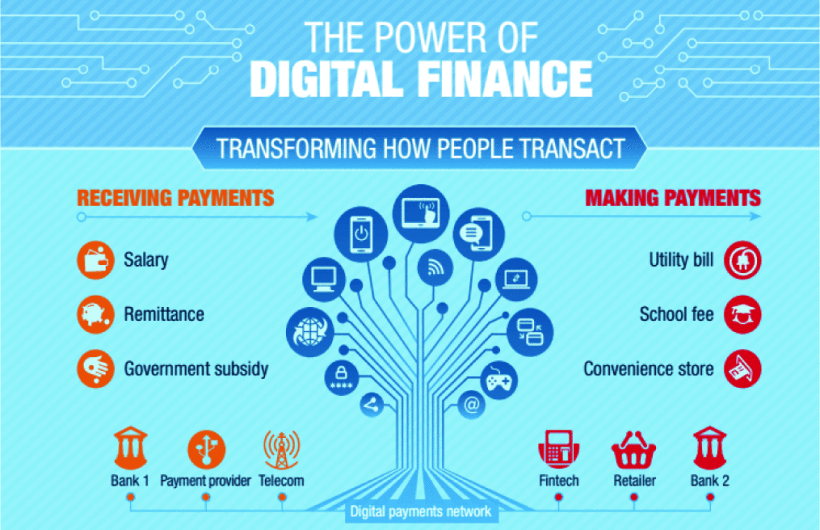
\includegraphics[width=0.90\textwidth]{src/resources/chapter-2-power-digital-finance.png}
    \caption{Transformasi Transaksi Finansial \textit{Fraud Detection System} \citep{8776857}}
    \label{fig:digital-finance}
\end{figure}

\vspace{10pt}

\subsection{Dasar Teori ke-4}

\blindtext

\blindtext

    %--------------------------------------------------------------------%
%
% Title         : Postgraduate Thesis LaTex template
% Author        : Ravi Vendra Rishika <ravi.vendra.rishika@gmail.com>
%
% Page          : Chapter 3
%
% It is developed especially for postgraduate students of :
%   Department of Informatics
%   Faculty of Intelligent Electrical and Informatics Technology
%   Sepuluh Nopember Institute of Technology (ITS)
%   Surabaya, Indonesia.
%
% This LaTex template is intended to make students easier
% to write master's degree thesis in LaTex using specific
% Department of Informatics of ITS' format.
%
%--------------------------------------------------------------------%

\chapter{METODOLOGI PENELITIAN}

Bab 3 merupakan penjelasan terkait metodologi penelitian yang digunakan
dalam penelitian ini, yang terdiri dari empat tahapan, yakni tahap pertama diawali dengan melakukan studi literatur terlebih dahulu. Tahap kedua adalah perancangan metode yang digunakan dalam penelitian. Tahap ketiga adalah implementasi metode, uji coba dan analisis hasil. Selanjutnya, tahap terakhir adalah penyusunan laporan penelitian.

Penjelasan detail terkait setiap bagian dari alur penelitian akan dijelaskan secara komprehensif pada subbab berikut ini.

\section{Studi Literatur}

\blindtext

\section{Perancangan Metode}

\blindtext

\section{Penyusunan Laporan Penelitian}

\blindtext

    %--------------------------------------------------------------------%
%
% Title         : Postgraduate Thesis LaTex template
% Author        : Ravi Vendra Rishika <ravi.vendra.rishika@gmail.com>
%
% Page          : Chapter 4
%
% It is developed especially for postgraduate students of :
%   Department of Informatics
%   Faculty of Intelligent Electrical and Informatics Technology
%   Sepuluh Nopember Institute of Technology (ITS)
%   Surabaya, Indonesia.
%
% This LaTex template is intended to make students easier
% to write master's degree thesis in LaTex using specific
% Department of Informatics of ITS' format.
%
%--------------------------------------------------------------------%

\chapter{EVALUASI DAN PEMBAHASAN}

\section{Tujuan Pengujian}

\blindtext

\section{Skenario Pengujian}

\blindtext

\section{Hasil Pengujian}

\blindtext

\section{Pembahasan}

\blindtext

    %--------------------------------------------------------------------%
%
% Title         : Postgraduate Thesis LaTex template
% Author        : Ravi Vendra Rishika <ravi.vendra.rishika@gmail.com>
%
% Page          : Chapter 5
%
% It is developed especially for postgraduate students of :
%   Department of Informatics
%   Faculty of Intelligent Electrical and Informatics Technology
%   Sepuluh Nopember Institute of Technology (ITS)
%   Surabaya, Indonesia.
%
% This LaTex template is intended to make students easier
% to write master's degree thesis in LaTex using specific
% Department of Informatics of ITS' format.
%
%--------------------------------------------------------------------%

\chapter{PENUTUP}

\blindtext

\section{Kesimpulan}

\blindtext

\section{Saran}

\blindtext

    
    % Bibliography
    %--------------------------------------------------------------------%
%
% Title         : Postgraduate Thesis LaTex template
% Author        : Ravi Vendra Rishika <ravi.vendra.rishika@gmail.com>
%
% Page          : Bibliography
%
% It is developed especially for postgraduate students of :
%   Department of Informatics
%   Faculty of Intelligent Electrical and Informatics Technology
%   Sepuluh Nopember Institute of Technology (ITS)
%   Surabaya, Indonesia.
%
% This LaTex template is intended to make students easier
% to write master's degree thesis in LaTex using specific
% Department of Informatics of ITS' format.
%
%--------------------------------------------------------------------%

\clearpage

% List of Bibliography
\addcontentsline{toc}{chapter}

\bibliography{bibliography}

\printbibliography


    % Indexes
    \appendix

    % \addcontentsline{toc}{part}{Lampiran}
    % \part*{Lampiran}

\end{document}
